\documentclass[10pt]{scrartcl}

\usepackage[utf8]{inputenc}
\usepackage{tabularx}
\usepackage[ngerman]{babel}
\usepackage[automark]{scrpage2}
\usepackage{amsmath,amssymb,amstext}
%\usepackage{mathtools}
\usepackage[]{color}
\usepackage[]{enumerate}
\usepackage{graphicx}
\usepackage{lastpage}
\usepackage[perpage,para,symbol*]{footmisc}
\usepackage{listings} 
\usepackage[pdfborder={0 0 0},colorlinks=false]{hyperref}
\usepackage[numbers,square]{natbib}
\usepackage{color}
\usepackage{colortbl}
\usepackage{listings}
\usepackage{a4wide}
\usepackage{xspace}
\usepackage{listings}
\usepackage{hyperref}

\lstset{numbers=left, numberstyle=\tiny, numbersep=5pt, breaklines=true, showstringspaces=false} 

%changehere
\def\titletext{TT1 Praktikum 1 \& 2 : Ausarbeitung}
\def\titletextshort{Praktikum 1 \& 2}
\author{Carsten Noetzel, Armin Steudte}

\title{\titletext}

%changehere Datum der Übung
\date{09.11.2011}

\pagestyle{scrheadings}
%changehere
\ihead{TT1, Schmidt}
\ifoot{Generiert am:\\ \today}

\cfoot{Carsten Noetzel, Armin Steudte}


\ohead[]{\titletextshort}
\ofoot[]{{\thepage} / \pageref{LastPage}}

\setlength{\parindent}{0.0in}
\setlength{\parskip}{0.1in}

\begin{document}
\maketitle

\setcounter{tocdepth}{3}
\tableofcontents
\listoffigures
%\lstlistoflistings

\section{Projektschritt 1 - Aufbau}
Im ersten Praktikumstermin wurden die Router konfiguriert und mit den nötigen Protokollen versehen. Die Versuchsdurchführung im zweiten Praktikumstermin wurde in Zusammenarbeit mit André Harms und Oliver Steenbruck durchgeführt und die Ergebnisse dokumentiert.\\
Der unter Abbildung \ref{fig:Aufbau} dargestellte Versuchsaufbau liegt den Versuchen zu Grunde. Hierbei wurde im Wechsel ein Router der Gruppe Noetzel, Steudte und der Gruppe Harms, Steenbruck aufgestellt und die Messungen zwischen den beiden äußersten Routern durchgeführt. Die Anzahl der Hops wurde mittels Tracert-Befehlen und bei OLSR über die Weboberfläche ermittelt. Dabei wurde angestrebt, dass die beiden äußersten Router über die beiden Router in  der Mitte kommunizieren, was sich in den Versuchen durch geschickte Positionierung der Router auch als erfüllbar erwies.

\begin{figure}[htbp]
	\centering	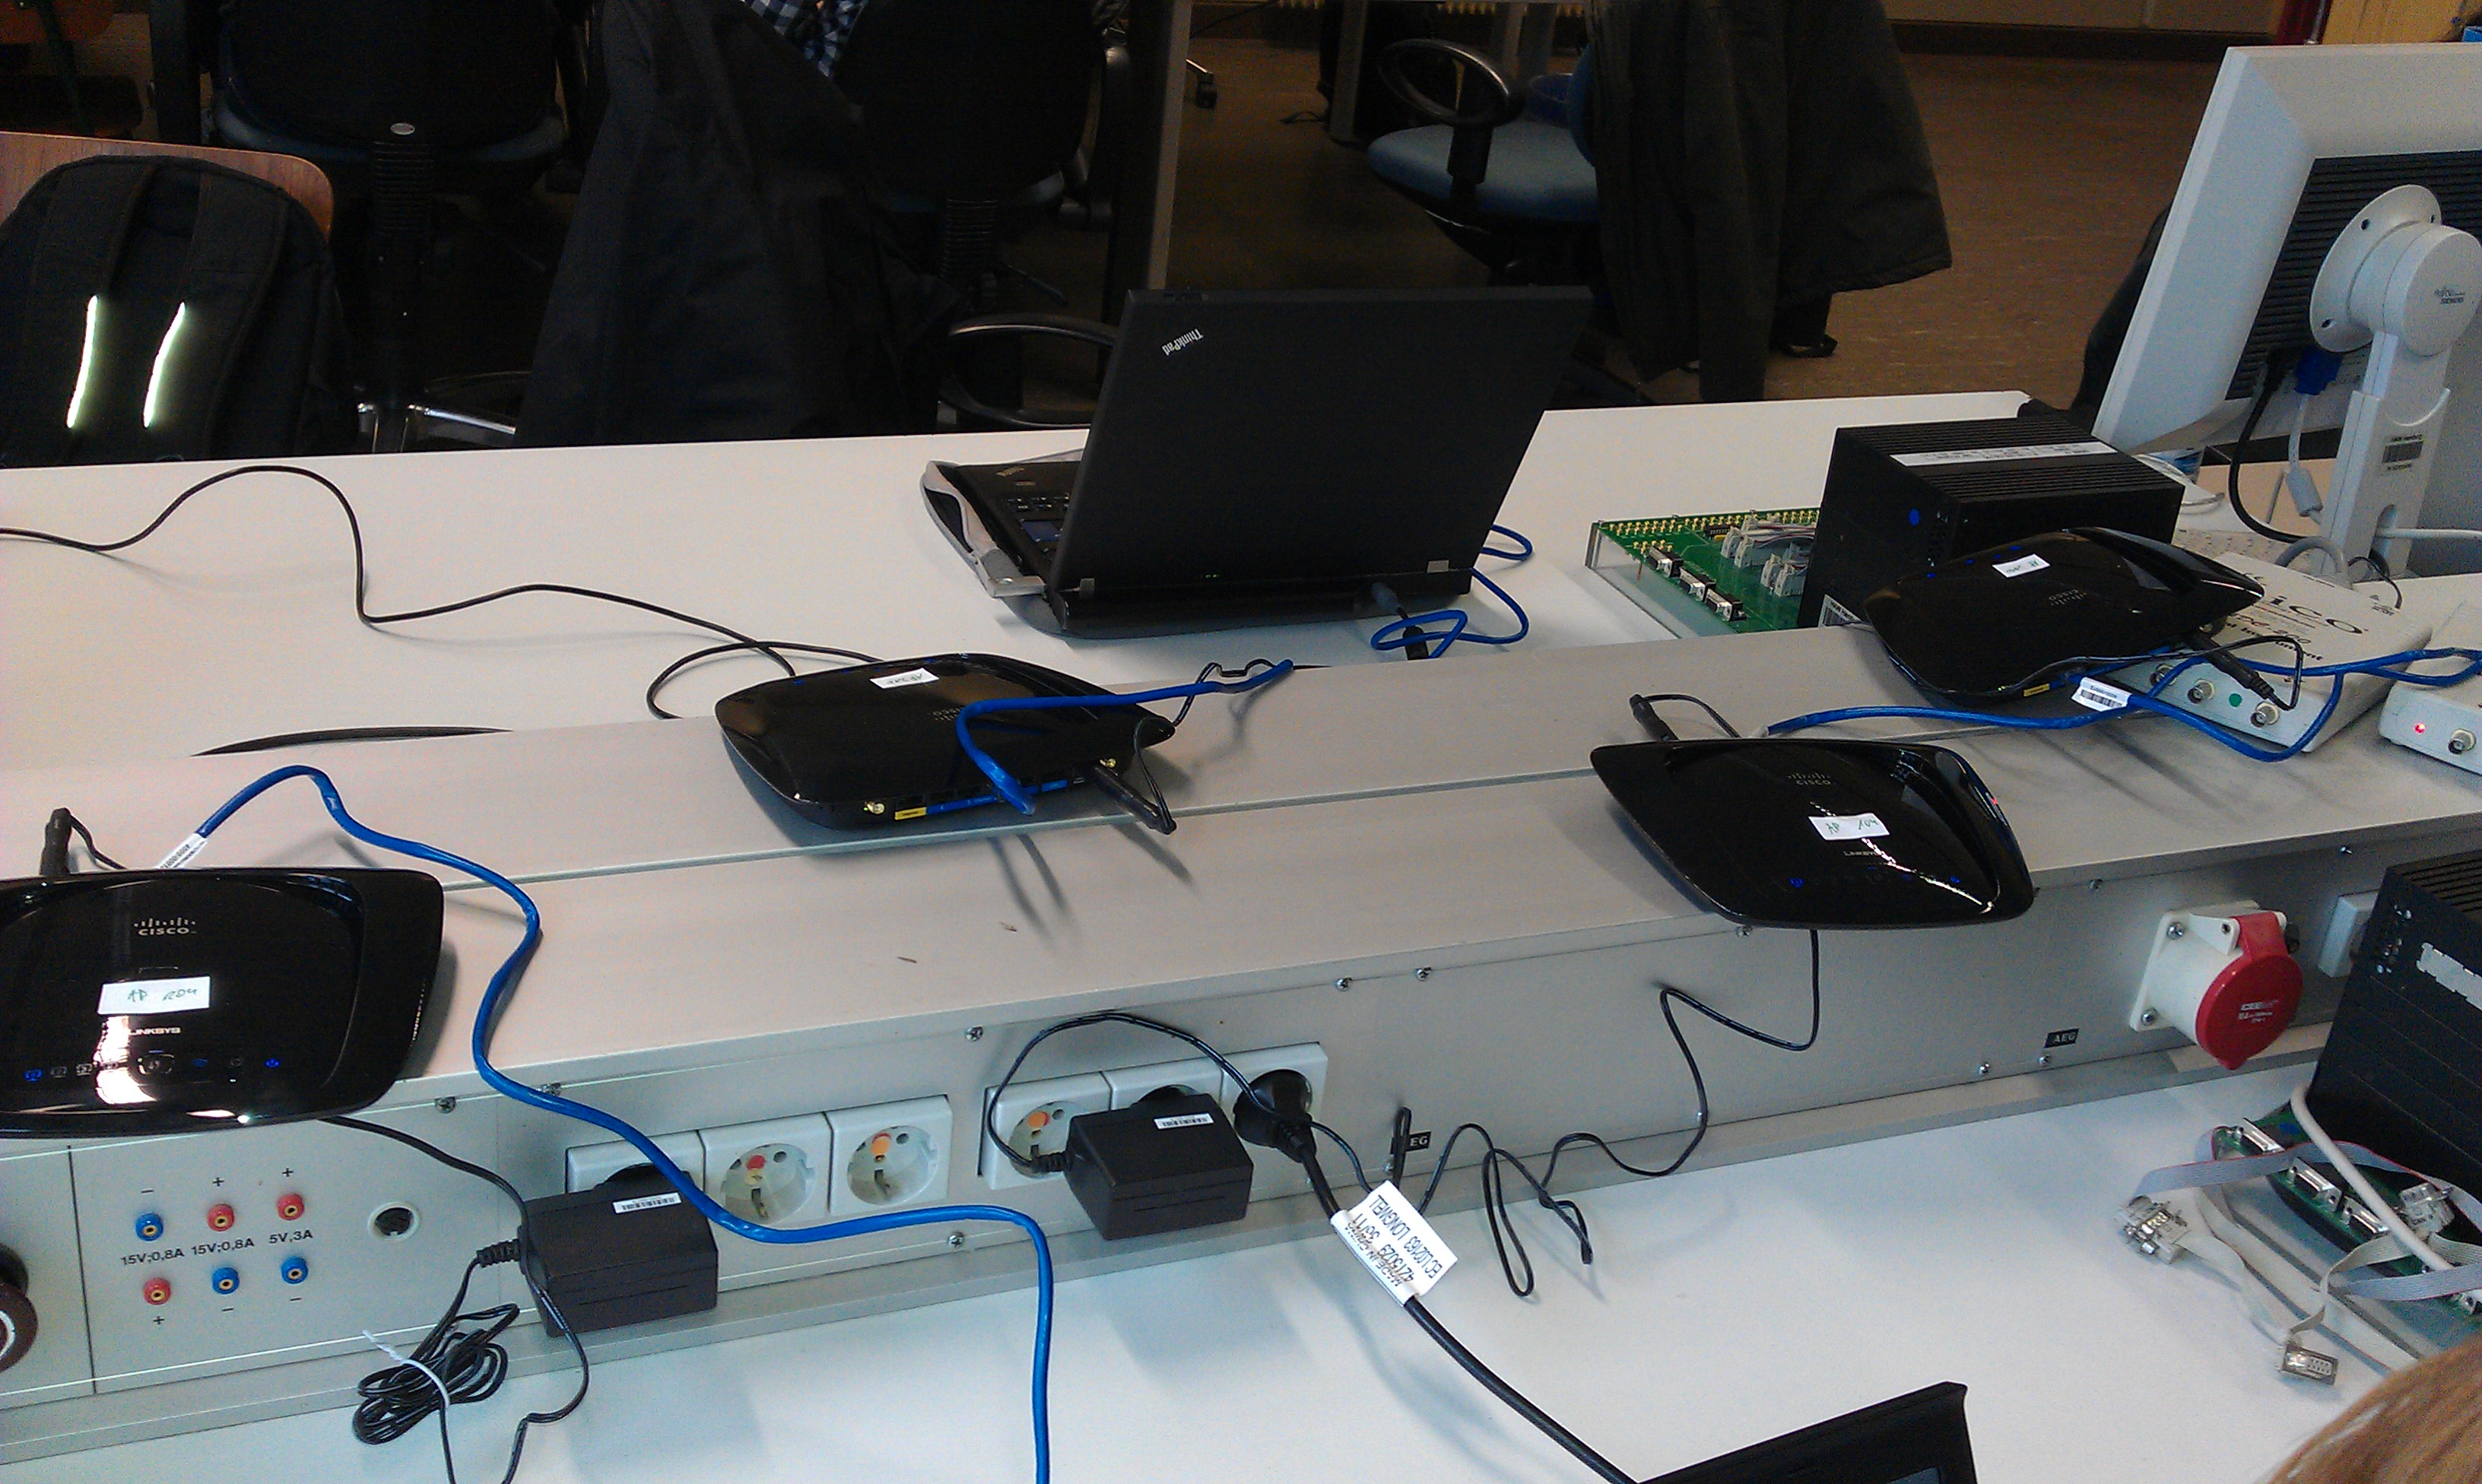
\includegraphics[width=1.0\textwidth]{Grafiken/AufbauBild.jpg}
	\caption{Versuchsaufbau mit 4 Routern}
	\label{fig:Aufbau}
\end{figure} 

\section{Projektschritt 2 - Vergleich Babel und OLSR}

\subsection{Babel}
\subsubsection{Informationsaustausch}
Jeder Router A hält beim Babel-Protokoll die Kosten zu einem Nachbarrouter B in der Form C(A, B) vor. Die Metrik einer Route bestimmt sich über die Summierung aller Kosten zwischen den Knoten die auf der Route liegen. Das Ziel des Algorithmus liegt darin für jede Quelle S einen Baum der Routen, mit den niedrigsten Metriken zu S zu berechnen.

Babel nutzt \textit{Hello-Messages} zur Durchführung des \textit{Neighbour-Discovery-Processes}.
Hello-Messages werden periodisch über alle Interfaces des Knoten gesendet um so die Nachbarknoten zu entdecken.\\
Zusätzlich werden Hello-Messages in Verbindung mit den \textit{IHY-Messages} (I Heard You Messages) genutzt, um die \textit{Bidirectional Reachability} und die Metrik zwischen Sender- und Empfängerknoten zu ermitteln.
Der Empfänger antwortet auf Hello-Messages mit den IHY-Messages. 
Diese erhalten die, mit Hilfe der Hello-Messages ermittelten, Laufzeitzeitverzögerungen aus Sicht des Senders der Hello-Messages.
Mit Hilfe der Laufzeitverzögerungen findet dann die Bewertung der Qualität der Links, sowohl in Sende- als auch Empfangsrichtung statt.



\subsubsection{Mesh - Konfiguration}
Die lokalen Mesh-Konfigurationen werden über einen verteilten Bellman-Ford Algorithmus berechnetet.\\
Hierzu hält jeder Router A zwei Werte vor, zum einen die geschätzte Distanz zu S (bezeichnet als D(A)) und den Next-Hop-Router zu S (bezeichnet als NH(A)). Zu Beginn des Informationsaustausches ist D(A)=unendlich und NH(A) ist nicht definiert.\\
Periodisch sendet jeder Knoten B ein Update seiner Routen an alle seine Nachbarn mit dem Inhalt D(B), welcher die Distanz zu S angibt. Erhält ein Nachbar A von B ein Update, so prüft A ob B für S als Next-Hop-Router eingetragen ist. Ist dies der Fall wird als Distanz D(A) die Summe aus C(A,B)( = Kosten von A nach B) und D(B)(= Kosten von B zu S) gesetzt. Damit ist im Knoten A die Metrik von A nach S über B aktualisiert.\\
Im Fall, dass B nicht als Next-Hop-Router für S auf A eingetragen ist, vergleicht A die Summe aus C(A,B)( = Kosten von A nach B) und D(B)(= Kosten von B zu S) mit dem gegenwärtigen Wert von D(A). Ist C(A,B)+D(B) kleiner als D(A) ist die angebotene Route besser als die bisher eingetragene und NH(A) wird auf B und D(A) auf C(A,B)+D(B) gesetzt.\\

Im Pseudocode sieht dies in etwa so aus:
\begin{lstlisting}
receiveRouteupdate(D(B)) from B for S
If NH(A) = B Then
	D(A) = C(A,B)+D(B)
Else
	If C(A,B)+D(B) < D(A) Then
		NH(A) = B
		D(A) = C(A,B)+D(B)
	EndIf
EndIf
\end{lstlisting}

Durch den Austausch der Updates wird Mesh-Konfiguration festgelegt und die Knoten wissen an welchen Knoten sie Pakete weiterleiten müssen, um ein bestimmtes Ziel mit möglichst geringen geschätzten Gesamtkosten zu erreichen.

\subsubsection{Loop-Verhinderungsstrategie}
Da es beim Bellman-Ford Algorithmus nach einer Topologieänderung und den damit verbundenen Updates zum \textit{Count-to-infinity}-Problem kommen kann, benötigt Babel eine Loop-Verhinderungs-Strategie.\\
Hierzu werden in Babel die sogenannten \textit{Feasibility Conditions} eingeführt. Dabei werden, erhaltene Routenaktualisierungen verworfen, wenn diese nicht beweisen können, dass die Annahme des Updates zu keinem Loop führen. Router A hält dazu eine \textit{Feasibility Distance} (bezeichnet als FD(A)) vor, welche als Wert die kleinste Distanz zu S enthält, die A jemals angeboten wurde. Ein Update von einem Nachbarn B ist zulässig (feasible), wenn die Metrik D(B) (= Kosten von B zu S) kleiner als As FD(A) ist.\\
Das diese Bedingung weniger restriktiv als die \textit{DSDV-Feasibility} ist, macht das Beispiel in Abbildung \ref{fig:Feasibility} deutlich. A kommt über B zu S, womit D(A)=FD(A)=2 ist. Da D(C)=1 und damit kleiner als FD(A) ist, ist eine alternative Route über C für A zulässig, auch wenn die Metrik C(A,C)+D(C) mit 5 schlechter als die aktuelle Route ist. Für den Fall das die Route über B abbricht kann so die Alternativroute genutzt werden.\\
Die \textit{DSDV-Feasibility} besagt, dass ein Update nur dann angenommen werden darf, wenn C(A,C)+D(C) kleiner oder gleich D(A) ist, wodurch die Alternativroute über C nicht zulässig wäre, da die DSDV-Bedingung nicht erfüllt ist (4+2 $<=$ 2).\\
Um zu zeigen, dass die \textit{Feasibility Condition} trotzdem noch Loop-Freiheit garantiert, sei zu beachten, dass wenn A ein Update von B akzeptiert D(B) nicht kleiner als FD(B) sein kann. Zudem gilt FD(B) ist kleiner als FD(A) da das Update für A zulässig ist und dieser es annimmt. Da diese Eigenschaft weiterhin erhalten bleibt, wenn A Updates versendet, ist sichergestellt, dass die Route keine Loops enthält.

\begin{figure}[htbp]
	\centering	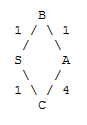
\includegraphics{Grafiken/Feasibility.png}
	\caption{Beispiel Feasabiliy Condition aus \href{http://tools.ietf.org/html/rfc6126}{RFC6126}}
	\label{fig:Feasibility}
\end{figure} 

Um zu verhindern, dass ein Router aufgrund fehlender zulässiger Routen ausgeschlossen wird, werden in Babel die Routen durchnummeriert. Ein Update von B an A ist damit zulässig, wenn entweder die \textit{Feasibility Condition} D(B)$<$FD(A) erfüllt ist und die das Update die gleiche Sequenznummer besitzt oder aber wenn die Sequenznummer des Updates höher ist.


\subsection{OLSR}
Bei \textit{OLSR} handelt es sich im Gegensatz zu Babel, wie der Name schon sagt, um einen Vertreter aus der Familie der Link-State-Routing Protokolle.
Dabei enthält OLSR gegenüber anderen Vertretern die Optimierung, dass die Knoten ihre Informationen nur an ihre \textit{Multipoint Relays (MPR)} senden müssen und diese das Verbreiten der Link-State Informationen übernehmen.
Somit ermöglicht OLSR ein effizientes \textit{Flooding} der Informationen.\\
OLSR ist proaktiv, wodurch Routen unmittelbar vorhanden sind wenn diese gebraucht werden.

\subsubsection{Informationsaustausch}
Wie auch in Babel tauschen Nachbarknoten bei OLSR \textit{Hello-Messages} aus.
Die Nachrichten haben dabei drei Aufgaben:
\begin{itemize}
	\item Erkennen von Links auf den Interfaces
	\item Neighbor Detection
	\item Bekanntgabe von MPRs
\end{itemize}
Zusätzlich werden auch noch \textit{TC Messages}, sogenannte \textit{Topology Control Messages}, über alle OLSR-Interface gesendet.
Sie enthalten Informationen über die lokale Topologie der Knoten und dienen zur Ermittlung der globalen Sicht auf das Netzwerk und dem Aufbau des Routing.
Sie werden, wie bereits erwähnt, nur durch die MPRs weitergeleitet.\\
Sollte OLSR auf mehreren Interfaces gleichzeitig laufen werden auch noch \textit{MID Messages (Main Adress and Multiple Interfaces)} gesendet, als zusätzliche Information zum Aufbau des Routing.
Da in unserem Fall die Router jeweils nur über die WLAN-Interfaces OLSR ausführten, wurden keine MID Messages generiert.\\

Bei der Bewertung der Qualität von Links kann auf zwei Methoden zurückgegriffen werden.
Standardmäßig wird die Anzahl an Hops als Grundlage für die Bewertung eines Links genutzt.
Außerdem existiert auch noch eine \textit{Link Quality Extension}, die die Hello-Messages nutzt um eine Wahrscheinlichkeit für den Paketverlust auf einem Link zu berechnen.
Pakete werde dann in diesem Fall über den Link mit der geringsten Wahrscheinlichkeit des Paketverlustes gesendet.\\
Im Praktikum wurde die Qualität der Routen mit der Anzahl an Hops gleichgesetzt, was der Standardkonfiguration des OLSR-Daemons entspricht.
Dieses ließ sich auch im Http-Status-Plugin des Daemons nachvollziehen (Abbildung einfügen).


\subsubsection{Mesh - Konfiguration}
Jeder Knoten im Netzwerk hält eine Routingtabelle mit folgenden Daten vor:

\begin{tabular}{l c c c c}
1. & R-dest-addr & R-next-addr & R-dist & R-iface-addr \\
2. &  R-dest-addr & R-next-addr & R-dist & R-iface-addr \\
3. & ,, & ,, & ,, & ,, \\
\end{tabular}

Jeder Eintrag der Liste gibt an, welches Ziel (R-dest-addr) über welchen Next-Hop-Router (R-next-addr) erreichbar ist und welches lokale Interface (R-iface-addr) dafür genutzt werden muss. Ferner wird die Distanz vom lokalen Router bis zum Ziel (R-dist) in der Tabelle vorgehalten.\\
Die Daten basieren auf Informationen der \textit{local link information dase} und der Topologie, wodurch die Routingtabelle jedes Mal neu berechnet werden muss, wenn sich diese Daten ändern. Für jedes Ziel im Netzwerk zu dem eine Route bekannt ist, wird ein Eintrag in der Tabelle vorgehalten.


\subsection{Vergleich Babel und OLSR}


\section{Projektschritt 3 - Vergleich der Übertragungsqualität}

\subsection{Versuchsaufbau}
Der Versuchsaufbau ist unter Abbildung \ref{fig:Aufbau} auf Seite \pageref{fig:Aufbau} zu sehen.\\
Die Router sind in folgender Reihenfolge aufgestellt (von links nach rechts): \textit{192.168.204.1}, \textit{192.168.210.1}, \textit{192.168.104.1} und \textit{192.168.110.1}. Die Messungen wurden über die äußerten Router durchgeführt, sodass sich mehrere Hops über die Router ergeben. Ein Tracert-Befehl von einem Client der mit dem Router \textit{192.168.104.1} verbunden ist, an einen Client der mit dem Router \textit{192.168.110.1} verbunden ist, ergibt die Route unter Abbildung \ref{fig:Route}.

\begin{figure}[htbp]
	\centering	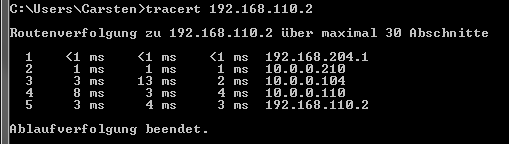
\includegraphics[width=0.5\textwidth]{Grafiken/Tracert.png}
	\caption{Route zwischen den Clients \textit{192.168.104.2} und \textit{192.168.110.2}}
	\label{fig:Route}
\end{figure}

Es wurde vor jedem Versuch sichergestellt, dass die Hop-Anzahl identisch ist, um vergleichbare Ergebnisse zu erzielen. Die Sendeleistung (TX-Power) wurde auf allen Geräten auf 1 gestellt, um möglichst viele Hops innerhalb unseres Versuchsaufbaus zu haben und nicht von anderen Gruppen gestört zu werden.

\subsection{Babel}
In diesem Abschnitt werden die Versuche vorgestellt, die mit dem Babel-Protokoll durchgeführt wurden.

\subsubsection{Versuch 1 - Übertragungsqualität}
Im ersten Versuch wurde die Übertragungsqualität von Babel gemessen, dabei wurden mit Hilfe des Programms \textit{JPerf} 10 MB über das UDP-Transportprotokoll, von Client \textit{192.168.110.2} an Client \textit{192.168.104.2} übertragen.\\
Die Ausgaben von JPerf sind unter Abbildung \ref{fig:JPerf_Babel_Protokoll} und Abbildung \ref{fig:JPerf_Babel_Graph} zu sehen.\\
Es ist zu erkennen, dass die Bandbreite zwischen 964 kbits/s und 612 kbits/s schwankt und sich ein Jitter zwischen 11,841 ms und 24,471 ms ergibt. Der Paketverlust liegt zwischen 4,3 \% und  95 \%. Echtzeitanwendungen die einen Jitter kleiner als 50 ms fordern, werden damit zwar erfüllt, jedoch ist die Paketverlustrate mit durchschnittlich 80 \% wesentlich höher als die geforderten 1 \%.\\
Der Grund für die geringe Bandbreite, den hohen Jitter und die hohe Verlustrate, liegt in der geringen Sendeleistung (Tx-Power = 1) der Router. Eine Erhöhung der Sendeleistung, kann diese Werte verbessern (siehe Versuch 3).

\begin{figure}[htbp]
	\centering	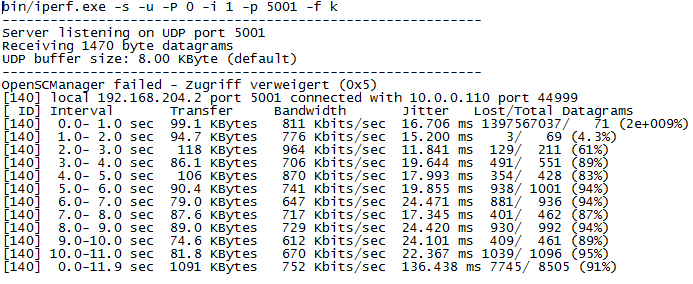
\includegraphics[width=0.8\textwidth]{Grafiken/Babel_TX1_Protokoll.png}
	\caption{JPerf Protokoll Babel}
	\label{fig:JPerf_Babel_Protokoll}
\end{figure}

\begin{figure}[htbp]
	\centering	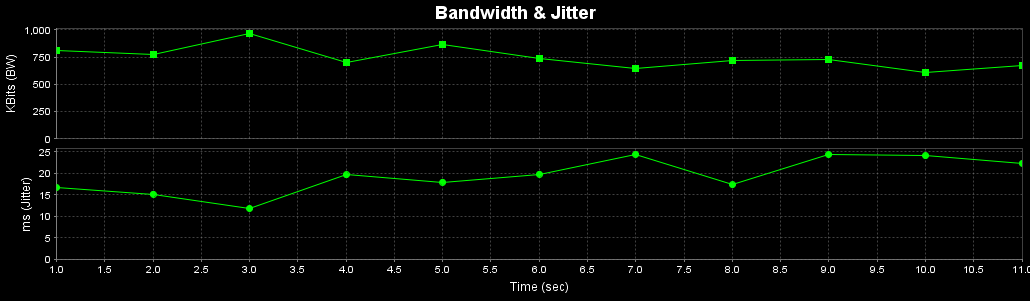
\includegraphics[width=1.0\textwidth]{Grafiken/Babel_TX1_Grafik.png}
	\caption{JPerf Bandbreiten und Jitter Graph - Babel}
	\label{fig:JPerf_Babel_Graph}
\end{figure}


\subsubsection{Versuch 2 - Failover}

\subsubsection{Versuch 3 - Erhöhung der Sendeleitung}
In diesem Versuch wurde lediglich die Sendeleistung des Router \textit{192.168.110.1} auf den Wert 11 gesetzt, um die Auswirkung einer erhöhten Sendeleistung zu untersuchen. Dabei wurde zunächst festgestellt, dass durch Erhöhung der Sendeleistung der Hop-Count zwischen den Clients um einen Hop abnimmt. Da der Router \textit{192.168.110.1} mit erhöhter Sendeleistung sendet, kann er Router \textit{192.168.210.1} direkt erreichen und muss nicht mehr über Router \textit{192.168.104.1} springen.\\
Es wurden wieder 10 MB mittels UDP von von Client \textit{192.168.110.2} an Client \textit{192.168.104.2} übertragen. Die Ergebnisse sind in Abbildung \ref{fig:JPerf_Babel_Protokoll_TX11} und Abbildung \ref{fig:JPerf_Babel_Graph_TX11} zu sehen.\\
Die Bandbreite liegt hierbei zwischen 4386 kbits/s und 5715 kbits/s und ist damit deutlich höher als im ersten Versuch. Auch beim Jitter, der in diesem Versuch zwischen 2,950 ms und 5,214 ms liegt, sind deutliche Verbesserungen festzustellen. Die Paketverlustrate liegt trotzdem noch zwischen 38 \% und 58 \%.\\
Trotz Erhöhung der Sendeleistung eines Routers, kann die Echtzeitanforderung mit einem maximalen Paketverlust von 1 \% nicht erfüllt werden. Es bleibt zu überprüfen, ob eine Erhöhung der Sendeleistung der anderen Router eine Verbesserung im Bereich der Verlustrate erwirkt.

\begin{figure}[htbp]
	\centering	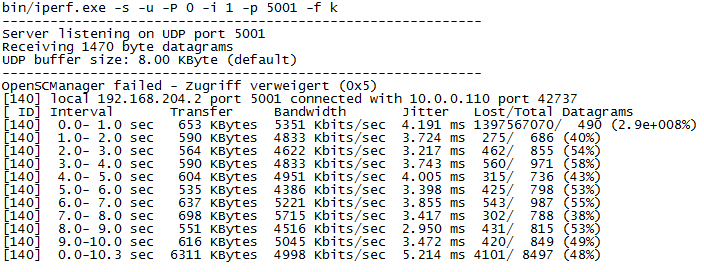
\includegraphics[width=0.8\textwidth]{Grafiken/Babel_TX11_Protokoll.png}
	\caption{JPerf Protokoll Babel mit erhöhter Sendeleistung}
	\label{fig:JPerf_Babel_Protokoll_TX11}
\end{figure}

\begin{figure}[htbp]
	\centering	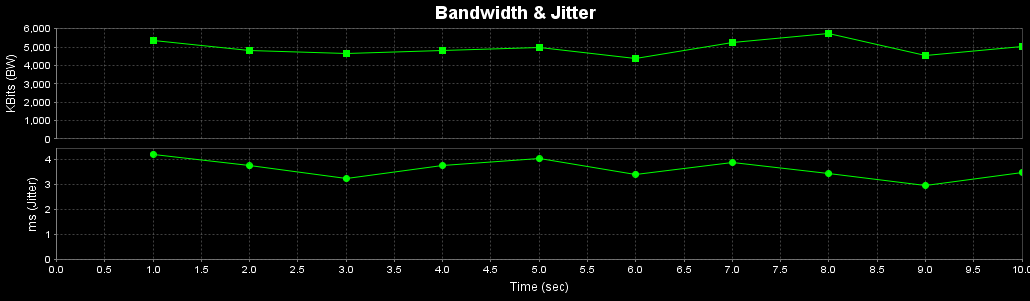
\includegraphics[width=1.0\textwidth]{Grafiken/Babel_TX11_Grafik.png}
	\caption{JPerf Bandbreiten und Jitter Graph - Babel mit erhöhter Sendeleistung}
	\label{fig:JPerf_Babel_Graph_TX11}
\end{figure}

\subsection{OLSR}
Dieser Abschnitt befasst sich mit den Versuchen, die mit dem OLSR-Protokoll durchgeführt wurden.

\subsubsection{Versuch 1 - Übertragungsqualität}
Im ersten Versuch wurden mittels JPerf 10 MB Daten von Client \textit{192.168.110.2} an Client \textit{192.168.104.2} übertragen. Als Transportprotokoll wurde hierbei UDP verwendet.

\begin{figure}[htbp]
	\centering	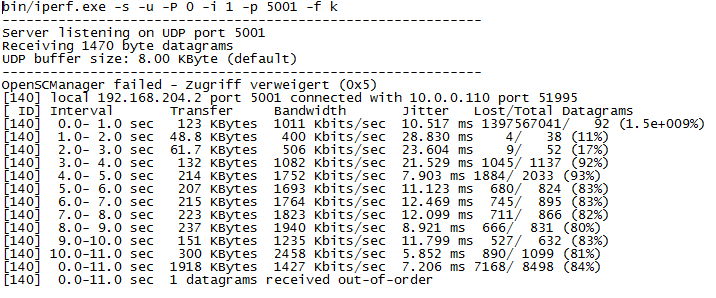
\includegraphics[width=0.8\textwidth]{Grafiken/OLSR_TX1_Protokoll.png}
	\caption{JPerf Protokoll OLSR}
	\label{fig:JPerf_OLSR_Protokoll}
\end{figure} 

\begin{figure}[htbp]
	\centering	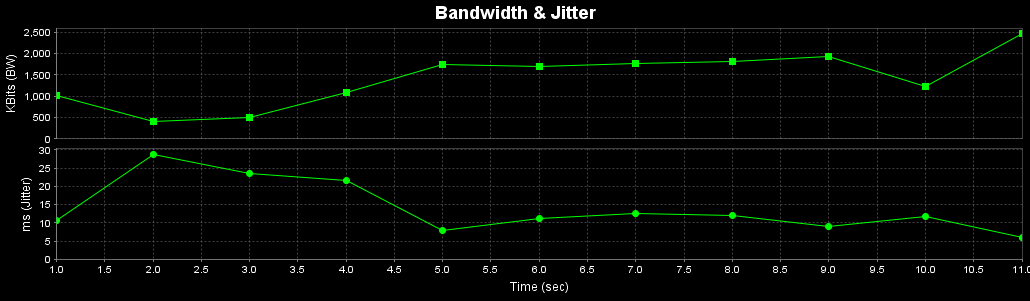
\includegraphics[width=1.0\textwidth]{Grafiken/OLSR_TX1_Grafik.png}
	\caption{JPerf Bandbreiten und Jitter Graph - OLSR}
	\label{fig:JPerf_OLSR_Graph}
\end{figure} 

\subsubsection{Versuch 2 - Failover}

\end{document}

